\chapter{Ensayos} % Main chapter title

\label{Chapter3} % Change X to a consecutive number; for referencing this chapter elsewhere, use \ref{ChapterX}


%----------------------------------------------------------------------------------------
%	Aquí se describen los distintos ensayos que se realizaron, y bajo que protocolo se
% trabajó. Mencionar los instrumentos utilizados.
% Se pueden incluir los ensayos realizados con los prograparticular aquellos que realizan curvas paramétricas.

%----------------------------------------------------------------------------------------
\section{Ensayos con marcos de prueba}
\label{Sección: Ensayos con marcos de prueba}
Se realizó el \textit{testbench} (marco de prueba) para cada entidad de diseño dentro del proyecto, para ensayar la respuesta de cada módulo a señales estímulo. Estas señales fueron representadas de manera de emular las señales correspondientes de aquellas para las que cada módulo se diseñó para manejar. Este tipo de ensayos se utilizó para observar la respuesta a estímulos de las diferentes entidades de la jerarquía de diseño yendo desde la entidad en el nivel más bajo a la entidad en el nivel más alto en la jerarquía.


\begin{itemize}
\item Jerarquía del CFAR:
	\begin{enumerate}
	\item FFD/Celda test
	\item
		\begin{enumerate}
		\item Celdas de guarda
		\item Celdas de referencia
		\end{enumerate}
	\item Comparador
	\item CFAR
	\item Contador CFAR
	\end{enumerate}
 
\item Jerarquía del Configurador
	\begin{enumerate}
	\item
		\begin{enumerate}
		\item Registro de entrada
		\item Registro de salida
		\end{enumerate}
	\item Sector fijo
	\item Procesador de presencias
	\item Ajuste de multiplicador
	\item Sector
	\item Sectorizador
	\item Configurador
	\end{enumerate}

\end{itemize}


\subsubsection{Flujo de simulación básico}


\begin{figure}
\centering
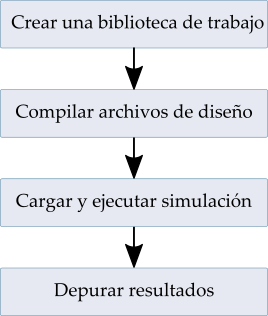
\includegraphics[scale=.7]{./Figures/flujo_simulacion.png}
\caption{Flujo de simulación básico}
\label{flujo_simulacion}
\end{figure}

El diagrama de la figura \ref{flujo_simulacion} muestra los pasos básicos para simular un diseño en ModelSim.

\begin{itemize}
\item
Creación de la biblioteca de trabajo:
En \textit{ModelSim}, todos los diseños se compilan en una biblioteca. Normalmente, una nueva simulación en \textit{ModelSim} comienza creando una biblioteca de trabajo llamada "trabajo", que es el nombre de biblioteca por defecto que utiliza el compilador como destino predeterminado para las unidades de diseño compiladas. Se creó, de este modo, dos bibliotecas, una para el cfar y otra para el configurador, cada una con todas las entidades de la jerarquía y sus correspondiente \textit{testbench}.

\item
Compilación del diseño:
Después de crear la biblioteca de trabajo, se compiló las unidades de diseño en ella. Esta compilación analiza cada archivo de forma individual y reporta, por ejemplo, errores de sintaxis o de falta de entidades en la librería que fueron instanciados en la entidad compilada. Estos reportes permiten realizar las correcciones necesarias en la entidad y/o arquitectura de un determinado archivo fuente. Sin embargo la compilación de todas las entidades no asegura el funcionamiento de todas ellas trabajando en conjunto (como un sistema) debido a que el análisis es a nivel individual.

\item
Carga del simulador con el diseño y ejecución de la simulación con el diseño compilado:
Una vez que la compilación resultó exitosa para todas las entidades de cada jerarquía se cargó el simulador con el \textit{testbench} asociado a cada entidad según el orden propuesto de ensayos descrito en la sección \ref{Sección: Ensayos con marcos de prueba}. Luego se estableció el tiempo de simulación en cero y se ejecutó en cada caso la simulación.

\item
Depuración sus resultados:
Se evaluó los resultados para cada simulación.
En algunos casos se escribió reportes dentro de la arquitectura VHDL por ejemplo, para determinar si en un \textit{process} se ingresó correctamente en todos los casos contemplados de alguna sentencia condicional. En otros se visualizó las formas de onda de las señales estímulo (entrada) y de respuesta (salida). En casos más complejos en donde no se obtuvo los resultados esperados y no se pudo determinar de "primera mano" la explicación a un determinado comportamiento, se utilizó el \textit{debugger} incorporado en \textit{ModelSim} para recorrer la ejecución en cada sentencia de las arquitecturas involucradas en el archivo fuente en cuestión.
\end{itemize}



    
    
   
    



\section{Ensayos con visores de netlist}

Se utilizó los visores de netlist \textit{RTL Viewer} y \textit{Technology Map Viewer}, descritos en la seccion \ref{seccion: Visores de netlist} del capítulo 2, para verificar la arquitectura de diseño de las entidades mencionadas en la sección \ref{Sección: Ensayos con marcos de prueba}.

El visor \textit{RTL Viewer} se utilizó para ver los resultados de la síntesis inicial y determinar si se creó la lógica necesaria y si el software interpretó correctamente la lógica y las conexiones. De esta manera se verificó el diseño visualmente.

En los casos en los que la simulación RTL arrojó un comportamiento inesperado, este visor fue útil para rastrear la lista de conexiones y asegurarse que las conexiones y la lógica en el diseño sean las esperadas. En caso de verificar la correcta interpretación de la herramienta de síntesis a este nivel, se analizó las etapas posteriores del proceso de diseño para investigar posibles violaciones de tiempo o problemas en el flujo de verificación en sí.

El visor \textit{Technology Map Viewer} se utilizó para ver los resultados al final de la compilación completa del diseño y determinar qué recursos fueron asignados en aquellos bloques en los que se observó un comportamiento erróneo durante la simulación en \textit{ModelSim}. Además, se utilizó para rastear conexiones entre entidades de diseño, sobre todo para verificar aquellas conexiones dedicadas a transportar la señal de un reloj a varios componentes.




\section{Ensayos con simulador y decodificador}
\label{Ensayos_simulador_decodificador}
Para verificar el funcionamiento del Configurador se utilizó un simulador. Dicho equipo se integró dentro de la FPGA con el objetivo de poder tener dos modos de configuración: uno en donde la señal a analizar proveniera del radar y otro en el que la señal proveniera del simulador. En el segundo modo de configuración, el equipo simuló todas las señales correspondientes a los radares primario y secundario, incluidos los ecos de estos sensores. Por defecto, en este modo se simulan 8 plots primarios y 8 plots secundarios por cada giro de antena, como se ilustra en la figura \ref{fig: plots simulador}. Este modo permite efectuar ensayos de mantenimiento y calibración sobre las distintas partes del Procesador Monoradar cuando no se dispone físicamente del sistema de radar.

Para ensayar el funcionamiento del configurador se diseñó un decodificador para recibir los datos de salida del mismo. Se dividió la cobertura en dos partes (agrupando 16 sectores en cada parte) y cada una se configuró con valores diferentes de algorítmo, multiplicador y coeficiente de ventana deslizante para verificar visualmente la confirmación (o no) de estos valores mediante el encendido (o apagado) de unos leds integrados en la placa.

Para determinar el crecimiento de la cantidad de targets detectados por el CFAR en un giro de antena, se utilizó el contador descrito en la sección \ref{subsubseccion: Contador CFAR}. Los cuatro bits más significativos de la cuenta se conectaron a cuatro leds integrados en la placa para verificar visualmente su variación a medida que el radar barrió la cobertura.

\begin{figure}
\centering
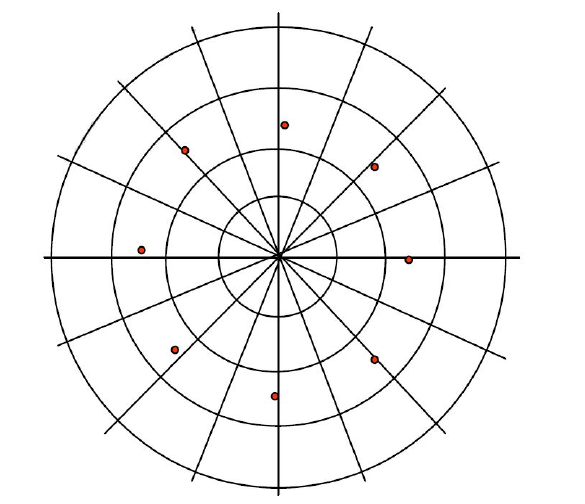
\includegraphics[scale=0.5]{./Figures/plots_simulador.png}
\caption{Distribución de plots de prueba}
\label{fig: plots simulador}
\end{figure}


\section{Ensayos con Procesador Monoradar preexistente}
\label{Ensayos_Procesador_Monoradar_preexistente}
Se utilizó un Procesador Monoradar preexistente para contrastar los datos arrojados por el Procesador Monoradar del que tanto el CFAR como el configurador descritos en este trabajo fueron parte. Para el CFAR se contrastó las ubicaciones de los plots detectados por ambos sistemas y se observó además la distribución de clutter. En el caso del configurador, se configuró varios sectores con diferentes valores de multiplicador para observar variación de clutter debido a los diferentes umbrales generados en estos sectores de la cobertura. Además para el configurador se varió el nivel de multiplicador  para algunos sectores, desde el nivel mínimo al máximo con el objetivo de visualizar en pantalla los límites de estos sectores.






